\section{Formål} 
I teknologidomænet analyseres QST som et teknologisk supplement til klinikerens vurdering af en patients henvisning til en TKA-operation. For at muliggøre dette kræves viden om både klinikerens vurdering og QST. Gennem problemanalysen er klinikernes vurdering undersøgt, mens teknologidomænet danner grundlag for viden om QST.\\
For at opnå viden om QST forventes en forståelse for teknologiens egenskaber, virkemåde samt begrænsninger. Heraf undersøges det oprindelige formål med QST, med henblik på at bestemme, hvordan denne er tilpasset og brugt i sammenhæng med TKA-operationer. Ydermere er det nødvendigt at vide hvad QST kan, hvordan denne fungerer, samt hvordan QST begrænses. Hermed er det muligt at vurdere hvordan og i hvilket omfang QST vil kunne fungere som supplement til klinikerens vurdering af en patients egnethed til en TKA-operation.\\
Da der er blevet tilegnet et kendskab til QST, er der grundlag for at undersøge og sammenligne QST med klinikerens vurdering. En sammenligning af QST med klinikerens metode er nødvendig for at kunne vurdere hvorvidt QST kan fungere som supplement hertil. 

\section{HTA spørgsmål}
Egenskaber ved QST:
\begin{enumerate}
	\item \textit{Hvad er det oprindelige anvendelsesområde for QST og hvordan er QST tilpasset knæartrose på nuværende tidspunkt?} %B0003, A0022}
	\item \textit{Hvordan virker QST?}  %B0001}
\end{enumerate}
Begrænsninger ved QST:
\begin{enumerate}[resume]
	\item \textit{Hvilke faktorer kan påvirke QST-resultaterne?}
\end{enumerate}
Sammenligning med nuværende metoder:
\begin{enumerate}[resume]
	\item \textit{Hvordan adskiller QST-teknologien og den nuværende medicinske teknologi sig fra hinanden?} %B0001, B0002}
\end{enumerate}

\section{Metode}
Litteratursøgningen benyttet til at kunne besvare HTA-spørgsmålene i TEC-domænet tager udelukkende udgangspunkt i den generelt skitserede metode (jævnfør \secref{litteratursogning}). Der er til besvarelse af domænets emner blevet søgt i følgende databaser; Primo, Pubmed, Medline og Embase. Dette har i litteratursøgningen bidraget til at specificere søgning til at kunne besvare det ønskede HTA-spørgsmål. Ved benyttelsen af databasernes syntax præfikser er det forud for søgningen taget højde for nogle af den pågældende søgnings inklusion- og eksklusionskriterier. Eksempelvis har et ekslusionskriterie været at udelukke andre sygdomme end artrose. Ligeledes har et inklusionskriterie været litteratur omhandlende QST-undersøgelser kun udført på personer med knæartose.  Dette har bidraget til at præcisere søgningen, inden den gerelle gennemgang af materiale. Igennem søgningerne er der til hvert HTA-spørgsmål blevet benyttet forskellige kombinationer af søgeord. Kombinationerne af forskellige søgeord har bidraget til at en bredere afsøgning af litteraturen inden for det specifikke HTA-spørgsmål. Dette har bidraget til at litteratursøgningen til det specifikke HTA-spørgsmål indebærer tilstrækkelig viden til netop at kunne besvare disse. \\
Der er i TEC-domænet kun benyttet videnskabelig litteratur af høj evidens i form af bøger og peer-reviewed materiale. Det er i TEC-domænet acceptabelt at supplere med non-peer reviewed-, ikke-publiceret materiale, fortroligt kommercielt materiale samt generelle internetsøgninger, hvilket i denne besvarelse ikke har været nødvendig. \citep{HTAcore} \\
Litteraturen der igennem den generelle udvælgelsesmetode, er fundet relevant, er blevet gennemlæst for at kunne tilegne sig viden til at besvare HTA-spørgsmålet. Al udvalgt materiale er gennemarbejdet, hvorefter dette er holdt op mod tilsvarende materiale. Dette har sikret en bred viden om teknologien, samt at forskelle og ligheder, litteratur imellem er blevet tydeliggjort. \\
Til besvarelse af HTA-spørgsmål (1) er der indsamlet litteratur omkring hvordan QST har udviklet sig. Denne litteratur danner grundlag for viden omkring det oprindelige formål for QST samt hvordan QST har udviklet sig til den form som kan anvendes til patienter med knæartrose. Herigennem vil det være muligt at bestemme præcis hvilke QST-parametre der skal undersøges for at besvare HTA-spørgsmål (2). Ved dette spørgsmål søges om litteratur hvor de fundne QST-parametre anvendes, og metoderne for undersøgelse af disse parametre beskrevet i de enkelte studier sammenlignes. \\
HTA-spørgsmål (3) besvares gennem viden fra de to foregående HTA-spørgsmål omkring hvordan undersøgelserne af de udvalgte QST-parametre udføres, samt litteratur omhandlende almindeligt forekomne begrænsninger ved undersøgelser. Det sidste HTA-spørgsmål, (4), besvares gennem en sammenfatning af viden fra problemanalysen samt de foregående HTA-spørgsmål.    
 
%\textbf{Tilføj følgende til metode: Hvordan har vi søgt(søgeord, kombinationer, inklussions og eksklusions, databaser), Hvilke slags litteratur er anvendt i domænet og nævn at det er høj evidens og at det ikke har været nødvendigt at bruge grå litteratur, selvom dette er acceptabelt i TEC-domænet. + forsøg at forklar hvordan du har benyttet litteraturen til at besvare spørgsmålene (Man har tilegnet sig en masse viden, sammenholdt dette og siger dette det samme?? + dette giver et stort overordnet billede af teknologien) GENERELT SKAL HELE DETTE METODE AFSNIT SKRIVES OM.}

\section{Teknologiens egenskaber}
\textit{I følgende afsnit undersøges teknologiens egenskaber. Dette gøres for at skabe et kendskab til QST's oprindelige formål samt hvilke QST-parametre der er relevante for patienter med knæartrose. Ligeledes beskrives undersøgelsesmetoden for de relevante QST-parametre.}

\subsection{Anvendelsesområde for QST}
I midten af det 19. århundrede blev der udviklet flere medicinske værktøjer til kvantitativ vurdering af sensation af stimuli. Vurderingselementerne omhandlede klassificering af tærskelværdier, tolerancer og stimuli-respons forhold. \citep{Yarnitsky1997} Forskerne i det sene 19. århundrede beskæftigede sig i større grad med tilstande, som ikke forvoldte smerter, og heraf blev de mest populære fund relateret til termisk- samt vibrationssensation. \citep{Yarnitsky1997} QST begyndte at blive anvendt specifikt til detektion af sensationsgrænser, hvilket senere specifik blev til detektion af smertertærskel og tolerancer. QST muliggør at undersøge tilstande ved benyttelse af andre typer stimuli. QST omfatter termisk, mekanisk, elektrisk, iskæmisk og kemisk påvirkning. \citep{Yarnitsky2006} De forskellige typer af stimuli bidrager til at kunne undersøge forskellige typer af nervefibre. Forsøgspersonernes reaktion på de forskellige stimuli kan klassificeres som værende af forringet eller forøget effekt, og visualiseres ofte igennem en visuel analog skala (VAS) \citep{Yarnitsky2006}. VAS benyttes til subjektiv bedømmelse af smerte, hvor smerteintensiteten angives som et tal mellem 0 og 10, hvor 0 er er ingen smerte og 10 er den værst tænkelige smerte \citep{smerter}. 

QST betegnes som en subjektiv vurderingsmetode, da det omfatter en subjektiv respons indenfor et psykofysik parameter til et kontrolleret stimuli. Den subjektive respons er på baggrund af, at patienten deltager frivilligt og af egen interesse. \citep{Mucke2016} Da vurderingsmetoden er subjektiv, kan resultatet blandt andet blive påvirket af distraktioner, kedsommelighed, mental træthed og forvirring. Ydermere kan en subjektiv respons bidrage til, at patienten bevidst fejlrapporterer på baggrund af en interesse i et bestemt resultat. \citep{Yarnitsky2006} Da QST er en subjektiv vurderingsmetode, bør behandlingen omfatte kvalitetskontrol, eksempelvis beståede repeterbarhed, reliabilitet og statistiske sammenhænge.

\subsubsection{Klinisk anvendelse af QST}
Generelt bliver QST anvendt til at klassificere sygdomme relateret til både til det centrale nervesystem (CNS) og det perifere nervesystem (PNS), heraf flere omhandlende sensationstab. Fastsættelsen af sensationstærskler relaterer sig til PNS, hvorimod smertekontrol relateres til CNS. \\ 
Ved benyttelse af QST relateret til diabetes ses det at 50\% af diabetikere har perifer neuropati, og ved anvendelse af en termisk parameter af QST, kan man tidligt i patogenesen identificere dette. Neuropati er ligeledes fundet ved flere patienter med nyresvigt, hvilket kan klassificeres igennem undersøgelse af vibration- og termisk sensation. \citep{Yarnitsky1997} \citep{Yarnitsky2006} \\
QST benyttes også til at klassificere smerter samt smertemekanismer, hvortil der er relateret en problemstilling. Da QST bygger på psykofysiske og psykologiske parametre opstår et problem i at der patienter imellem er forskel i smerteopfattelse og smertereaktion. \citep{Yarnitsky1997} Forståelsen af disse smertemønstre, kan med den korrekte QST tilgang, bidrage til at kunne forudsige responsen på en given interaktion. \citep{Yarnitsky2006} Ydermere kan QST i smerteregi, klinisk blive benyttet til at lave kvantitative sammenligninger mellem forskellige grupperinger \citep{Arendt-Nielsen2009}. \\
Generelt benyttes QST-resultater ikke, som det eneste resultat til at stille en diagnose. Dette er på baggrund af tidligere nævnte årsager relateret til det subjektive aspekt i metoden. \citep{Yarnitsky2006}

\subsubsection{Tilpasning af QST til knæartrose}
QST bliver i  knæartroseregi forsøgt benyttet til at skabe en association imellem præoperativ smertesensation og udviklingen af kronisk postoperativ smerte. Dette ses også ved den øgede kirurgiske interesse for benyttelse af teknologien. Der ses et potentiale i anvendelsen af præoperative QST-undersøgelser, som prædiktion for omfanget af kroniske postoperative smerter. \citep{Wylde2013} Ved hjælp af QST kan klinikeren undersøge denne smertesensation igennem flere forskellige parametre eksempelvis, tryk-smerte tærskelen, kulde/varme-tærskel og tolerance, kulde-smerte rating, temporal summation og konditioneret smertemodulation. \citep{Cornelius2015} Dette er blot et uddrag af parametre, der kan testes for at skabe en smertesensationsprofil. Ved benyttelse af mange parametre vil QST være omfattende og tidskrævende, hvilket kan antages at være problematisk i et klinisk regi. Dette skaber en begrænsning i benyttelse af QST, og dermed bør kun diagnostisk relevante parametre blive benyttet. \citep{Nielsen2009} En sammenfatning af flere studier antyder, at central sensibilisering har betydning for udviklingen af kroniske postoperativesmerter efter en TKA-operation \citep{Suokas2012}. Central sensibilisering formodes at opstå som følge af langvarig smertepåvirkning, som et resultat af de degenererende forandringer, der sker i et led på grund af knæartose. \citep{Arendt-Nielsen2015b} Princippet bag formodningen illustreres på \figref{fig:widespread_sens} \citep{Graven-Nielsen2010} . 

\begin{figure}[H] 
	\begin{center}
		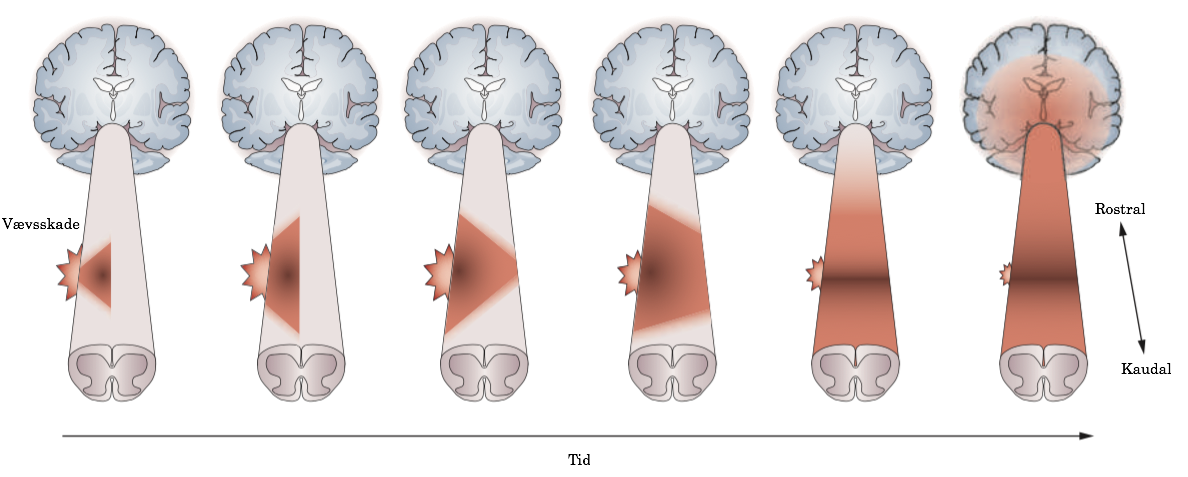
\includegraphics[width=0.7\textwidth]{figures/dHTAanalyse/widespread_sens}
	\end{center}
	\caption{Figuren viser, hvordan en en vævsskade som forårsager lokal smerte, udvikles til central sensibilisering. Vævsskaden med dets relaterede smertereceptorer formodes at skabe central sensibilisering som et resultat af langvarig smertepåvirkning. \citep{Graven-Nielsen2010}} 
	\label{fig:widespread_sens} 
\end{figure} \vspace{-.25cm}

Efter en succesfuld TKA-operation normaliseres den centrale sensibilisering i nogle tilfælde, mens for patienter med kroniske postoperative smerter forbedres den centrale sensibilisering ikke i samme grad. Central sensibilisering kan undersøges ud fra følgende QST-parametre, tryksmertetærskel (PPT), temporal summation af smerte (TSP) og konditioneret smertemodulation (CPM). \citep{Arendt-Nielsen2015b} Flere studier har ligeledes undersøgt hvilke parametre, som er diagnostisk relateret til udviklingen af kroniske postoperative smerter. Her er den største konsensus ligeledes, at QST-parametrene med størst diagnostisk relevans for knæartrose, er nedsat PPT, faciliteret TSP og nedsat CPM. Alle disse QST parametre kan profileres igennem mekanisk QST. \citep{Petersen2015} \citep{Petersen2016} \citep{Wylde2015b} \\
I et studie af \citer{Petersen2016}, blev knæartrosepatienter grupperet efter deres QST-resultater vedrørende TSP og CPM. Disse inddelinger resulterede i at hverken TSP eller CPM, som enkeltstående måleparameter, statistisk kan benyttes som indikerende faktorer for en patients postoperative resultat. Studiet indikerer heraf at patienter både med faciliteret TSP og nedsat CPM, har mindre smertelindring end andre patienter. Dette resultat understreger at multible QST-parametre bør benyttes for at QST kan opfylde dets kliniske formål. \citep{Petersen2016} Flere studier indikerer at udbredt hyperalgesi kan være en prædiktivt faktor, for en patients kroniske postoperative smerter. \citep{Petersen2016} \citep{Wylde2013} Dette understøttes også i studiet af \citer{Wylde2016c}, hvis resultater indikerer at patienter med en sværere grad af knæartrose og mere udbredt hyperalgesi, får et mindre godt udbytte af TKA, end patienter med mindre udbredt hyperalgesi. Dette resulterer i at udbredt hyperalgesi kan være en prædiktiv faktor, men resultaterne er af svag statistisk evidens. \citep{Wylde2016c}\\
På baggrund af ovenstående analyse, ses en indikation på at QST-parametrene, PPT, TSP og CPM kan anvendes til identificering af patienter i risiko for at udvikle kroniske postoperative smerter. Heraf vil den videre analyse udelukkende omhandle QST-parametrene PPT, TSP og CPM.

\subsection{Undersøgelse af PPT, TSP og CPM}
De tre QST-parametre PPT, TSP og CPM kan testes ved forskellige typer stimuli. PPT testes mekanisk, mens TSP og CPM kan testes mekanisk, kemisk, elektrisk eller termisk. Oftest anvendes mekanisk stimuli i form af tryk. \citep{Suokas2012} \citep{Yarnitsky2006} Det er ifølge \citep{Imai2016}, blevet påvist at ved udførsel af CPM er pålideligheden størst ved anvendelse af mekanisk tryk stimuli, sammenlignet med benyttelse af kulde og varme \citep{Imai2016}. Heraf vil omtalte QST parametre fremtidigt tage udgangspunkt i mekanisk stimuli i form af tryk. Til trykstimuli kan udstyr fra Somedic eller NociTech anvendes \citep{Wylde2015b} \citep{Petersen2016}. 

Ved test af PPT undersøges det, om patienten har en forstærket reaktion på tryk. Dette kan gøres både på områder i umiddelbar nærhed af det påvirkede knæ og på områder, som er længere væk fra knæet. En lav PPT-værdi, og dermed højere sensitivitet for stimuli, i området omkring det påvirkede knæ antyder perifer sensibilisering, mens en lav PPT-værdi i områder væk fra det påvirkede knæ antyder central sensibilisering. \citep{Suokas2012} Det påførte tryk stiger indtil patienten begynder at opfatte trykket som smertefuldt, og angiver dette ved eksempelvis tryk på en knap. PPT defineres som det påførte tryk, da patienten angav, at trykket blev smertefuldt, og angives dermed i kPa. Oftest gentages målingen tre gange, hvorefter gennemsnittet af de tre målinger anvendes som patientens PPT-værdi. \citep{Petersen2015} \citep{Wylde2015b} 

En forhøjet TSP kan antyde central sensibilisering, da reguleringen af TSP i neuroner er formindsket ved central sensibilisering. \citep{Arendt-Nielsen2015b} Hermed reagerer personer med central sensibilisering stærkere på gentagende stimuli end personer som ikke har central sensibilisering, hvilket illustreres på \figref{fig:TSP_rask_syg}. \citep{Arendt-Nielsen2015b} 

\begin{figure}[H] 
	\begin{center}
		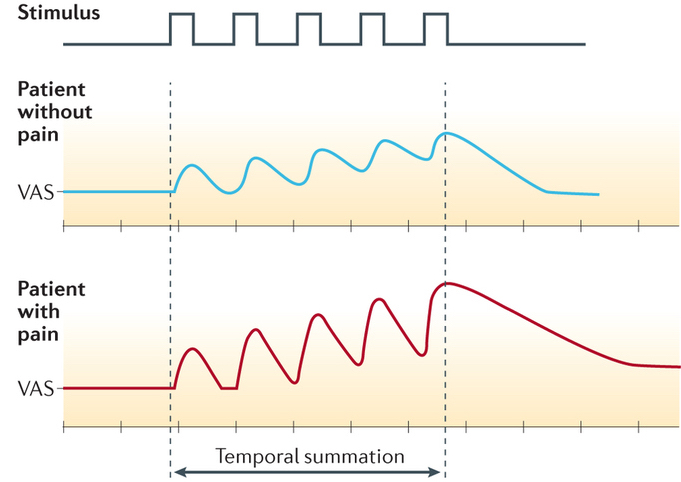
\includegraphics[width=0.6\textwidth]{figures/dHTAanalyse/TSP_rask_syg.jpg}
	\end{center}
	\caption{Figuren viser, hvordan patienter med faciliteret TSP responderer anderledes på gentagende samme stimuli, end patienter uden faciliteret TSP. \citep{Reynolds2016}} 
	\label{fig:TSP_rask_syg} 
\end{figure} \vspace{-.25cm}

For at undersøge en patients TSP påføres patienten gentagne tryk med samme intensitet, med tilsvarende intervaller. I studiet af \citer{Petersen2016} blev patienten tilført tryk på et sekunds varighed efterfulgt af en pause på et sekund. Patienten blev i alt tilført 10 tryk. For hvert tryk angav patienten smerten på ud fra VAS, og TSP udregnes som gennemsnittet af VAS for de første fire tryk trukket fra gennemsnittet af VAS for de sidste tre tryk. \citep{Petersen2016} TSP kan ligeledes udregnes ved at trække VAS-scoren for det sidste stimuli fra VAS-scoren for det første stimuli. \citep{Petersen2015} 

Descenderende smerteregulering er en betydende faktor for udviklingen af central sensibilisering. Den descenderende smerteregulering regulerer neuronernes reaktion på stimuli, og består af en balance mellem inhiberende og exciterende signaler. For personer med normal descenderende smerteregulering er denne hovedsageligt inhiberende. Ved central sensibilisering forskubbes balancen i den descenderende smerteregulering, således neuronernes reaktion på stimuli ikke inhiberes på samme niveau som tidligere. Denne forskydning i balancen kan ske enten ved, at færre inhiberende signaler sendes eller, at flere exciterende signaler sendes til neuronerne. \citep{Arendt-Nielsen2015b} Den descenderende smerteregulering undersøges ved CPM. Ved test af CPM udsættes patienten for smertestimuli et sted på kroppen, mens PPT måles et andet sted på kroppen, som benævnes teststedet. Før den smertefulde stimuli tilføres patienten bliver PPT målt på teststedet. \citep{Petersen2016} Den smertestimuli der tilføres patienten kan eksempelvis være termisk eller mekanisk. CPM defineres som forskellen i PPT på teststedet før og efter den smertefulde stimuli er tilført et andet sted på kroppen. \citep{Petersen2015} 

\section{Teknologiens begrænsninger}
\textit{Efter beskrivelse af de tre QST-parametre, PPT, TSP og CPM undersøges begrænsningerne for undersøgelsesmetoderne. Hermed bestemmes eventuelle svage punkter ved hver af parametrene.}

\subsection{Begrænsende faktorer ved benyttelse af QST}
Ved benyttelsen af QST som supplement til klinikerens beslutning, bør teknologiens begrænsende faktorer vurderes. Som nævnt er den største konsensus omkring diagnostisk relevante QST-parametre PPT, TSP og CPM. \\
Ved benyttelsen af PPT, bør metodens udførsel undersøges. Det kan forestilles, at hvis de tre målinger til at danne PPT-værdien, udføres med for kort et interval, kan der opstå komplikationer i form af en carry-over effekt. En carry-over effekt som et bias i et klinisk forsøg er når der opstår fejlresultater på baggrund af videreførsel af tidligere stimuli-respons, til fremtidige forsøg. For PPT-målinger vil denne carry-over effekt ske, hvis transmitterstoffer som blev udskilt fra neuroner ved første stimuli, ikke er blevet reabsorberet før et nyt stimuli tilføres. \citep{martini} Hvis PPT-målingerne tages med for kort interval, kan det tænkes at der vil opstå en carry-over effekt, som kan resultere i en falsk PPT-værdi. Herfor er det vigtigt at overveje hvor lang tid der går mellem hver måling, således carry-over effekten så vidt muligt undgås. \citep{Porta2008} 

For at kunne benytte QST som et led i den diagnostiske process, kræves det at klinikeren har adgang til et sæt normativ data til klassificering af anormale tilstande. Det normative datasæt skal bestå af normale tærskler og tolerancer, samt anormale tærskler og tolerancer, førend klinikeren kan adskille patientgrupper fra hinanden. Udviklingen af sådanne normative datasæt er nødvendig førend en mulig implementering. Ved fremadrettet benyttelse af normative data kræves det at den samme metode benyttes. Hvis ikke den samme metode benyttes kan det forestilles, at resultaterne vil afvige fra det normative datasæt, og heraf skabe falsk negative/positive resultater. Heraf vil standardiserede normative datasæt bidrage til at skabe pålidelige resultater, og dermed højne teknologiens sensitivitet og specificitet. \citep{Yarnitsky1997} Problematikken vedrørende benyttelsen af normativ data ses ligeledes i studiet af \citer{Petersen2016}, hvor forsøgspopulationen inddeles i grupperinger vurderet på baggrund af arbitrære valg. Forfatterene pointerer tilmed i studiet, at en normativ inddeling af patienter er nødvendig, og bør optimeres og gøres generaliserbar, førend implementering af QST. \citep{Petersen2016} Forbedringen skal bidrage til at optimere sensitiviteten og specificiteten og dermed øge muligheden for at kunne forudsige om en given patient får kroniske postoperative smerte efter TKA. 

\section{Sammenligning med nuværende metoder}
\textit{I følgende afsnit analyseres det hvordan QST-parametrene ud fra de foregående fund, kan bidrage til vurderingsgrundlaget. Dette gøres ved at undersøge samspillet mellem QST og den medicinske teknologi i form af klinikerens nuværende vurdering.}

\subsection{Sammenspil mellem QST og klinisk vurdering} 
Den nuværende metode til udvælgelse af knæartrosepatienter til en TKA-operation bygger på kirurgers observationer og samtaler med patienten, og er dermed en kvalitativ vurdering. \citep{Troelsen2012} \citep{skou2016} Den eneste kvantitative parameter som anvendes ved den nuværende metode er radiologiske fund, der ikke altid er indikative for patientens oplevelse af smerte \citep{Leary2016}. Ved anvendelse af QST tilføjes en kvantitativ målemetode som er en mulig prædiktor for udvikling af kroniske postoperative smerter. Såfremt QST har den ønskede effekt, vil tilføjelsen styrke vurderingsgrundlaget idet en beslutningsmetode, som bygger på både kvalitative og kvantitative observationer. Dette giver et mere udførligt helhedsbillede end en beslutningsmetode som kun er bygget på den ene af de to slags observationer. \citep{Gronmo2012} \\
Herudfra kan QST fungere som et supplement til klinikerens udvælgelse på baggrund af dens kvantitative karakteristika, og mulighed for tilføjelse af ny viden til klinikerens beslutningsgrundlag. Dette kræves dog, at QST nøjagtigt kan identificere patienterne med forhøjet risiko for udvikling af kroniske postoperative smerter.   

\section{Delkonklusion}
\textit{I dette afsnit sammenfattes de vigtigste pointer fra TEC-analysen, og sættes i sammenhæng hvorledes disse bidrager til besvarelse af problemformuleringen.}

QST blev oprindeligt udviklet til undersøgelse af forsøgspersoners sensation af stimuli. Siden er der blevet udviklet en række forskellige protokoller, der har hver sit formål. Den QST-protokol som er anvendelig til undersøgelse af muskuloskeletale smerter, og hermed kroniske postoperative smerter, indeholder parametre som kan antyde central sensibilisering. Disse tre parametre er PPT, TSP og CPM. PPT kan kun undersøges ved anvendelse af tryk, mens TSP og CPM kan undersøges ved flere forskellige stimuli, men oftest ved anvendelse af mekanisk tryk. Det er ikke påvist at PPT, TSP og CPM som enkeltstående parametre kan anvendes til identificering af patienter som ville udvikle kroniske postoperative smerter, men resultater fra et studie antyder at patienter med forhøjet TSP og inhiberet CPM, har flere postoperative smerter end andre patienter. Undersøgelserne der omhandler de tre QST-parametre har en række begrænsninger. En af disse begrænsninger er at der, på nuværende tidspunkt, ikke er fundet normative værdier for de tre parametre. Uden normative værdier er det ikke muligt for klinikeren at vurdere om patienten har anormale værdier eller ej. Ligeledes er et problem med QST at undersøgelsernes resultater afhænger af patientens subjektive svar og reaktioner. Dette ekskluderer patienter som ikke har evne til at forstå instrukserne, fra undersøgelserne. Herudover kan patienters, både bevidste og ubevidste, bias påvirke undersøgelsernes resultater. Dette svækker ligeledes pålideligheden af QST-resultater, da det ikke kan kontrolleres om resultatet er sandt, da det er en subjektiv bedømmelse fra patienten. \\
På trods af begrænsningerne ved anvendelse af QST, indikerer flere studier at QST har potentialet til at styrke klinikerens vurderingsgrundlag. For at dette er muligt kræves det at begrænsningerne ved undersøgelserne omhandlende de diagnostisk relevante QST-parametre nedbringes. Hvis dette udbedres kan QST-undersøgelserne styrke vurderingsgrundlaget, idet der ved anvendelse af QST tilføjes en kvantitativ metode til klinikerens overvejende kvalitative metode. Samlet set bør QST på et givent tidspunkt når udviklingen og optimeringen er udarbejdet, kunne fungere som supplement til klinikeren, og heraf øge kvaliteten af den nuværende behandling.


